\documentclass{article}

%% Denote paragraphs with vertical space rather than indenting (not critical)
\usepackage{parskip}

%% Support for URL in introductory text (not needed for main example)
\usepackage{url}

%% *** Enable TikZ ***
\usepackage{tikz}

%% *** TikZ library ***
\usetikzlibrary{calc,math}

\begin{document}

%% Introductory Text
Example 4.12 from the book\\
\emph{Unlocking LaTeX Graphics: A Concise Guide to Ti$k$Z/PGF and PGFPLOTS}.\\
For more information, visit \url{https://latex-graphics.com}.
\par\bigskip

%% *** START OF EXAMPLE CODE ***
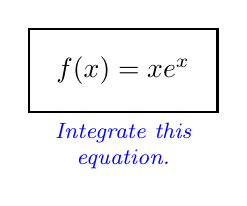
\begin{tikzpicture}
  \node[draw,thick,inner sep=1em] (A) {$f(x)=xe^x$};
  \path let \p1=(A.south west),\p2=(A.south east) in (\p1) -- (\p2)
  node[text width=0.8*(\x2-\x1), blue, midway, below,
    font=\footnotesize\itshape,align=flush center]
  {Integrate this equation.};
\end{tikzpicture}
%% *** END OF EXAMPLE CODE ***

\end{document}
